\documentclass[a4paper,11pt]{report}
\usepackage[french]{babel}
\usepackage[T1]{fontenc}
\usepackage[utf8]{inputenc}
\usepackage{lmodern}
\usepackage{microtype}
\usepackage{hyperref}
\usepackage{tabulary}
\usepackage{framed}
\usepackage{fancyhdr}
\usepackage{amsmath}
\usepackage{bbm}
\usepackage{graphicx}
\usepackage{pst-all}
\usepackage{xcolor}

%\usepackage{nopageno}

\newcommand{\latin}[1]{\textit{#1}}

\pagestyle{empty}

\pagestyle{fancy}
\fancyhead{}
\renewcommand{\headrulewidth}{0.5pt}
\fancyhead[R]{\textit{\nouppercase{\rightmark}}}
\fancyfoot{}
\renewcommand{\footrulewidth}{0.5pt}
\fancyfoot[L]{\textit{\nouppercase{\leftmark}}}
\fancyfoot[R]{\thepage}
  
\begin{document}
	\begin{titlepage}
		\vspace*{\stretch{2}}
		\begin{center}
			\large\bfseries\itshape Stage ETE 2015\\
		\end{center}
		\noindent\rule{\linewidth}{3pt}

		\begin{center}
			\Huge\bfseries\itshape Description du système\\
		\end{center}
		
		\noindent\rule{\linewidth}{3pt}
		\begin{center}
			\bfseries
			\large F-PHT \\
			\large Un système d'index de filtres de Bloom pour la recherche d'information par mots clés
		\end{center}
		\vspace*{\stretch{2}}
		\begin{center}
			Réalisé par \textbf{DOAN} Cao Sang \\
			Encadrant: M. \textbf{MAKPANGOU} Mesaac, Regal
		\end{center}
		\vspace*{\stretch{0.5}}
		\begin{center}
			30 Juin 2015
		\end{center}
	\end{titlepage}

\tableofcontents

\chapter{Vue globale}
\section{Prefix Hash Tree (PHT)}
	Un arbre préfixe est un arbre numérique ordonné qui est utilisé pour stocker une table associative où les clés sont généralement des chaînes de caractères. Contrairement à un arbre binaire de recherche, aucun nœud dans le trie ne stocke la chaîne à laquelle il est associé. C'est la position du nœud dans l'arbre qui détermine la chaîne correspondante\footnote{Wikipédia}.
	
	Pour tout nœud, ses descendants ont en commun le même préfixe. La racine est associée à la chaîne vide. Des valeurs ne sont pas attribuées à chaque nœud, mais uniquement aux feuilles et à certains nœuds internes se trouvant à une position qui désigne l'intégralité d'une chaîne correspondant à une clé.
	
	\begin{figure}[!htbp]
	\centering
	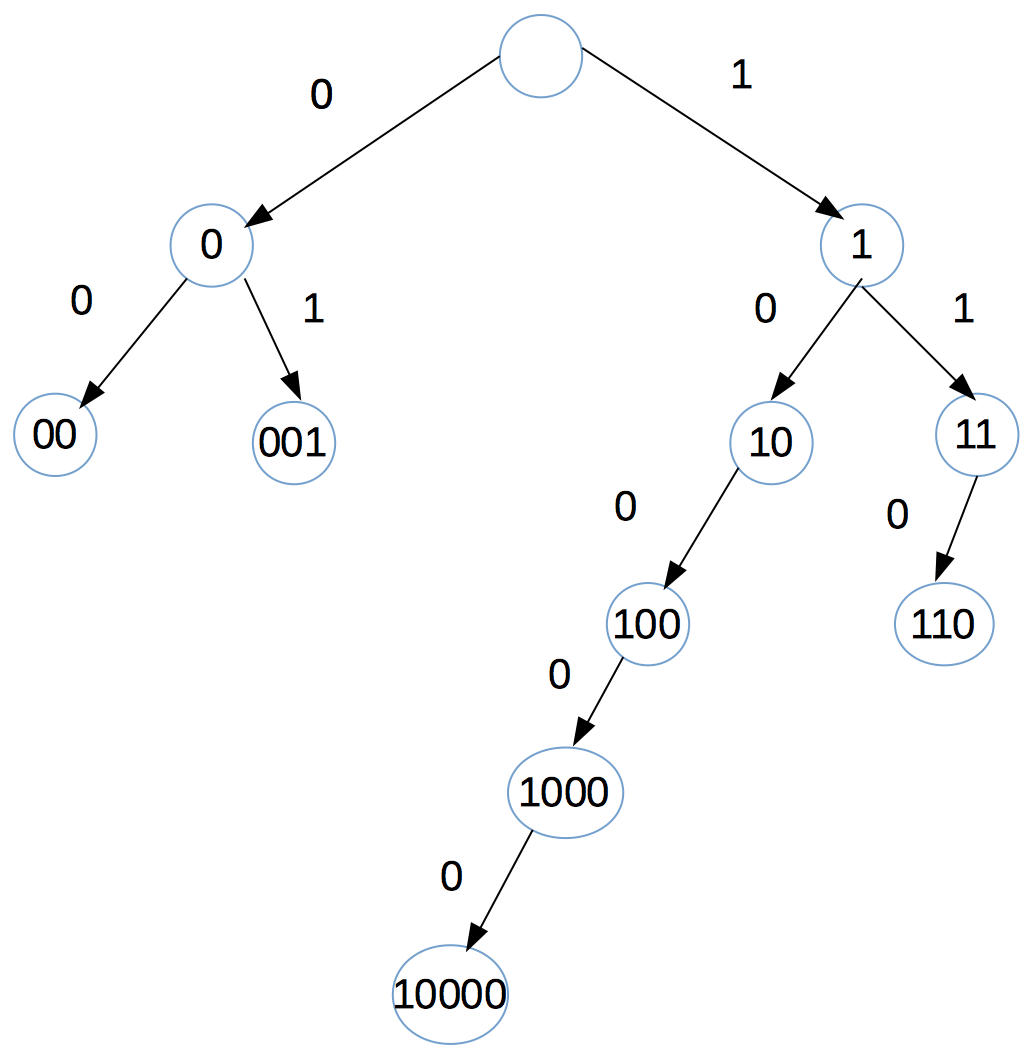
\includegraphics[width=12cm]{PHT.eps}
	\caption{Un arbre préfixe}
\end{figure}	

\newpage

\section{Fragment}
	On considère un filtre de Bloom de taille \textit{m}. Le système découpe ce filtre en \textit{f} fragments de taille identique. Par convention, les fragments sont numérotés de \textit{0} à \textit{f-1}, en commençant par le fragment le plus à gauche. L'identifiant de chaque fragment est défini de façon unique.
	
		Par exemple, \textit{m = 16}, \textit{f = 4}.

	\begin{table}[!h]
		\centering		
		\begin{tabular}{|l|*{14}{c|}r|}
		\multicolumn{1}{c}{{\scriptsize 15}} &\multicolumn{1}{c}{}&\multicolumn{1}{c}{}&\multicolumn{1}{c|}{}&\multicolumn{1}{c}{}&\multicolumn{1}{c}{}&\multicolumn{1}{c}{}&\multicolumn{1}{c|}{}&\multicolumn{1}{c}{}&\multicolumn{1}{c}{}&\multicolumn{1}{c}{}&\multicolumn{1}{c|}{}&\multicolumn{1}{c}{}&\multicolumn{1}{c}{}&\multicolumn{1}{c}{}&\multicolumn{1}{c}{{\scriptsize 0}}\\
		\hline
			1 & 0 & 0 & 0 & 1 & 1 & 0 & 1 & 0 & 0 & 0 & 0 & 1 & 0 & 1 & 0 \\
		\hline
		\end{tabular}
		\caption{Exemple le filtre de Bloom}
		\label{fragment/filtredeBloom}
	\end{table}

	\begin{table}[!h]
		\centering		
		\begin{tabular}{|l|*{2}{c|}r|}
		\hline
			1 & 0 & 0 & 0 \\
		\hline
		\end{tabular}
		\caption{Exemple la valeur de fragment \textit{f = 0}}
		\label{fragement/exemple1}
	\end{table}

	\begin{table}[!h]
		\centering
		\begin{tabular}{|l|c|c|r|}
		\multicolumn{1}{c}{}&\multicolumn{1}{c}{}&\multicolumn{1}{c}{}\\
		\hline
			1 & 0 & 1 & 0 \\
		\hline
		\end{tabular}
		\caption{Exemple la valeur de fragment \textit{f = 3}}
		\label{fragement/exemple2}
	\end{table}
	
\newpage

\section{F-PHT}
	F-PHT est une sorte d'arbre préfixe, il utilise  les filtres de Bloom  de taille \textit{m} comme clés de stockage. Cet arbre utilise l'identifiant d'un fragment de filtre de Bloom à la place de préfixe. Chaque nœud de l'arbre stocke un ensemble de couple /textbf{<prefix, identifiant>} avec \textbf{préfix} est la valeur d'un fragment de rang \textbf{i} et \textbf{identifiant} est soit l'identifiant d'un nœud soit null. Si \textbf{identifiant} est égal à null, \textbf{prefix} est un filtre de Bloom. Sinon, ce couple désigne où sont stockés les filtres de Bloom ayant \textbf{prefix} comme valeur du fragment de rang \textbf{i}, où \textbf{i} correspond au niveau de ce nœud dans l'arbre.

	Chaque nœud contient une liste \textbf{RouteEntry}, qui contient les couples stockés par ce nœud. Chaque nœud stocke au plus $\gamma$ couples, avec $\gamma$ inférieur ou éqal à $2^{\frac{m}{f}}$.

\end{document}









